\newif\ifshowsolutions
\showsolutionstrue
\newcommand{\solutionname}{Answer}
\documentclass{article}
\usepackage{listings}
\usepackage{amsmath}
%\usepackage{subfigure}
\usepackage{subfig}
\usepackage{amsthm}
\usepackage{amsmath}
\usepackage{amssymb}
\usepackage{graphicx}
\usepackage{mdwlist}
\usepackage{geometry}
\usepackage{titlesec}
\geometry{margin=1in}
\geometry{headheight=2in}
\geometry{top=2in}
\usepackage{palatino}
\usepackage{mathrsfs}
\usepackage{fancyhdr}
\usepackage{paralist}
\usepackage{todonotes}
\setlength{\marginparwidth}{2.15cm}
\usepackage{tikz}
\usetikzlibrary{positioning,shapes,backgrounds}
\usepackage{float} % Place figures where you ACTUALLY want it
\usepackage{comment} % a hack to toggle sections
\usepackage{ifthen}
\usepackage{needspace} % keep a question's header on the same page as its first lines
\usepackage{mdframed}
\usepackage{verbatim}
\usepackage[strings]{underscore}
\usepackage{listings}
\usepackage{bbm}
\usepackage[colorlinks=true, linkcolor=blue, filecolor=magenta, urlcolor=cyan, pdftitle={CS 155 Miniproject 2}]{hyperref}

\rhead{}
\lhead{}

\renewcommand{\baselinestretch}{1.15}

% Shortcuts for commonly used operators
\newcommand{\E}{\mathbb{E}}
\newcommand{\Var}{\operatorname{Var}}
\newcommand{\Cov}{\operatorname{Cov}}
\newcommand{\Bias}{\operatorname{Bias}}
\DeclareMathOperator{\argmin}{arg\,min}
\DeclareMathOperator{\argmax}{arg\,max}

% do not number subsection and below
\setcounter{secnumdepth}{1}

% hide section numbers (the counter still steps, so question letters restart each part)
\titleformat{\section}{\normalfont\Large\bfseries}{}{0pt}{}

% custom format subsection
\titleformat*{\subsection}{\large\bfseries}

% set up the \question shortcut
\newcounter{question}[section]
\newenvironment{question}[1][]
  {\refstepcounter{question}\par\addvspace{1em}\needspace{6\baselineskip}\textbf{Question~\Alph{question}\!
    \ifthenelse{\equal{#1}{}}{}{ [#1 points]}: }}
    {\par\vspace{\baselineskip}}

\newcounter{subquestion}[question]
\newenvironment{subquestion}[1][]
  {\refstepcounter{subquestion}\par\medskip\textbf{\roman{subquestion}.\!
    \ifthenelse{\equal{#1}{}}{}{ [#1 points]:}} }
  {\par\addvspace{\baselineskip}}

\titlespacing\section{0pt}{12pt plus 2pt minus 2pt}{0pt plus 2pt minus 2pt}
\titlespacing\subsection{0pt}{12pt plus 4pt minus 2pt}{0pt plus 2pt minus 2pt}
\titlespacing\subsubsection{0pt}{12pt plus 4pt minus 2pt}{0pt plus 2pt minus 2pt}


\newenvironment{hint}[1][]
  {\textbf{Hint: }}{}

\providecommand{\solutionname}{Solution}   % the student template sets this to "Answer"
\ifshowsolutions
  \newenvironment{solution}[1][]
    {\par\medskip \begin{mdframed}\textbf{\solutionname~\Alph{question}#1:} }
    {\medskip\end{mdframed}\medskip}
  \newenvironment{ecsolution}
    {\par\medskip \begin{mdframed}\textbf{\solutionname{} (extra credit):} }
    {\medskip\end{mdframed}\medskip}
  \newenvironment{subsolution}[1][]
    {\par\medskip \begin{mdframed}\textbf{Solution~\Alph{question}#1.\roman{subquestion}:} }
    {\medskip\end{mdframed}\medskip}
\else
  \excludecomment{solution}
  \excludecomment{subsolution}
  \excludecomment{ecsolution}
\fi

\graphicspath{{../figs/}}

\chead{%
  {\vbox{%
      \large
      Machine Learning \& Data Mining \hfill
      Caltech CS/CNS/EE 155 \hfill \\[1pt]
      Miniproject 2: Image Features for Classification\hfill
      Released: November 10 \\
    }
  }
}

\begin{document}
\pagestyle{fancy}

\section{Overview}

\noindent
\textbf{Important Note.} The goal of this project is \textbf{not} to get the highest
accuracy. You will be graded mainly on the depth and completeness of your analysis.

\begin{itemize}
\item In this project you will classify CIFAR-10 images and study how much the
  features you feed a classifier matter, compared with the classifier itself.
  In Part 1 you use PCA features computed from raw pixels. In Part 2 you use features
  from a large model pretrained on images and text. In Part 3 you classify images
  without training on any labeled images at all. In Part 4 you probe a failure of that
  last approach.

\item All starter code is in the accompanying Google Colab notebook:
  \url{https://drive.google.com/file/d/1-3Jo6hA1v9mWjSg9qQQ3FGEOu7gN2ayu/view?usp=sharing}.
  Open it in Colab and make your own copy (\texttt{File $\rightarrow$ Save a copy in
  Drive}) before you start, since the shared notebook is view-only. Work in your copy and
  fill in every \texttt{\# TODO}. Use a GPU runtime
  (\texttt{Runtime $\rightarrow$ Change runtime type $\rightarrow$ T4 GPU}).

\item The report is due \textbf{Tuesday, November 17, at 11:59 PM PST} via Gradescope.
  Write it in the provided LaTeX template, which has an answer box for every written
  question. Include the plots and numbers each question asks for, as well as any additional
  evidence that would support your analysis. Implementation questions are
  graded from your notebook and need no written answer.

\item Submit your code by \textbf{sharing a link to your Colab notebook in Question 0
  of the template}. Set sharing permissions to at least ``Anyone with the link can view''.
  \textbf{Links that cannot be run by TAs will not be counted as turned in.} Check
  your link in an incognito window before submitting.

\item You may work in groups of 2--4.

\item We split CIFAR-10 into a training set (its 50,000 training images) and a holdout
  set (its 10,000 test images). Train only on the training set. Every accuracy you
  report, and every choice you make (number of PCA components, architecture, prompts),
  uses the holdout set.
\end{itemize}

\noindent\textbf{Question 0: Colab link.} Paste the link to your Colab notebook. Set sharing to
``Anyone with the link can view'', and check that it opens in an incognito window.
\begin{mdframed}
Your link here. % e.g. \url{https://colab.research.google.com/drive/...}
\end{mdframed}

\pagebreak
\section{Part 1: PCA Features (35 points)}

Throughout this project we classify images from
CIFAR-10\footnote{\url{https://www.cs.toronto.edu/~kriz/cifar.html}}, a standard image
classification dataset. It contains 60{,}000 color images of size $32 \times 32$, split evenly across
10 classes: airplane, automobile, bird, cat, deer, dog, frog, horse, ship, and truck.
The classes do not overlap. For example, ``automobile'' covers cars, and ``truck''
covers only big trucks. Figure~\ref{fig:cifar} shows examples from each class. We use
the 50{,}000 training images as our training set and the 10{,}000 test images as our
holdout set.

\begin{figure}[H]
\centering
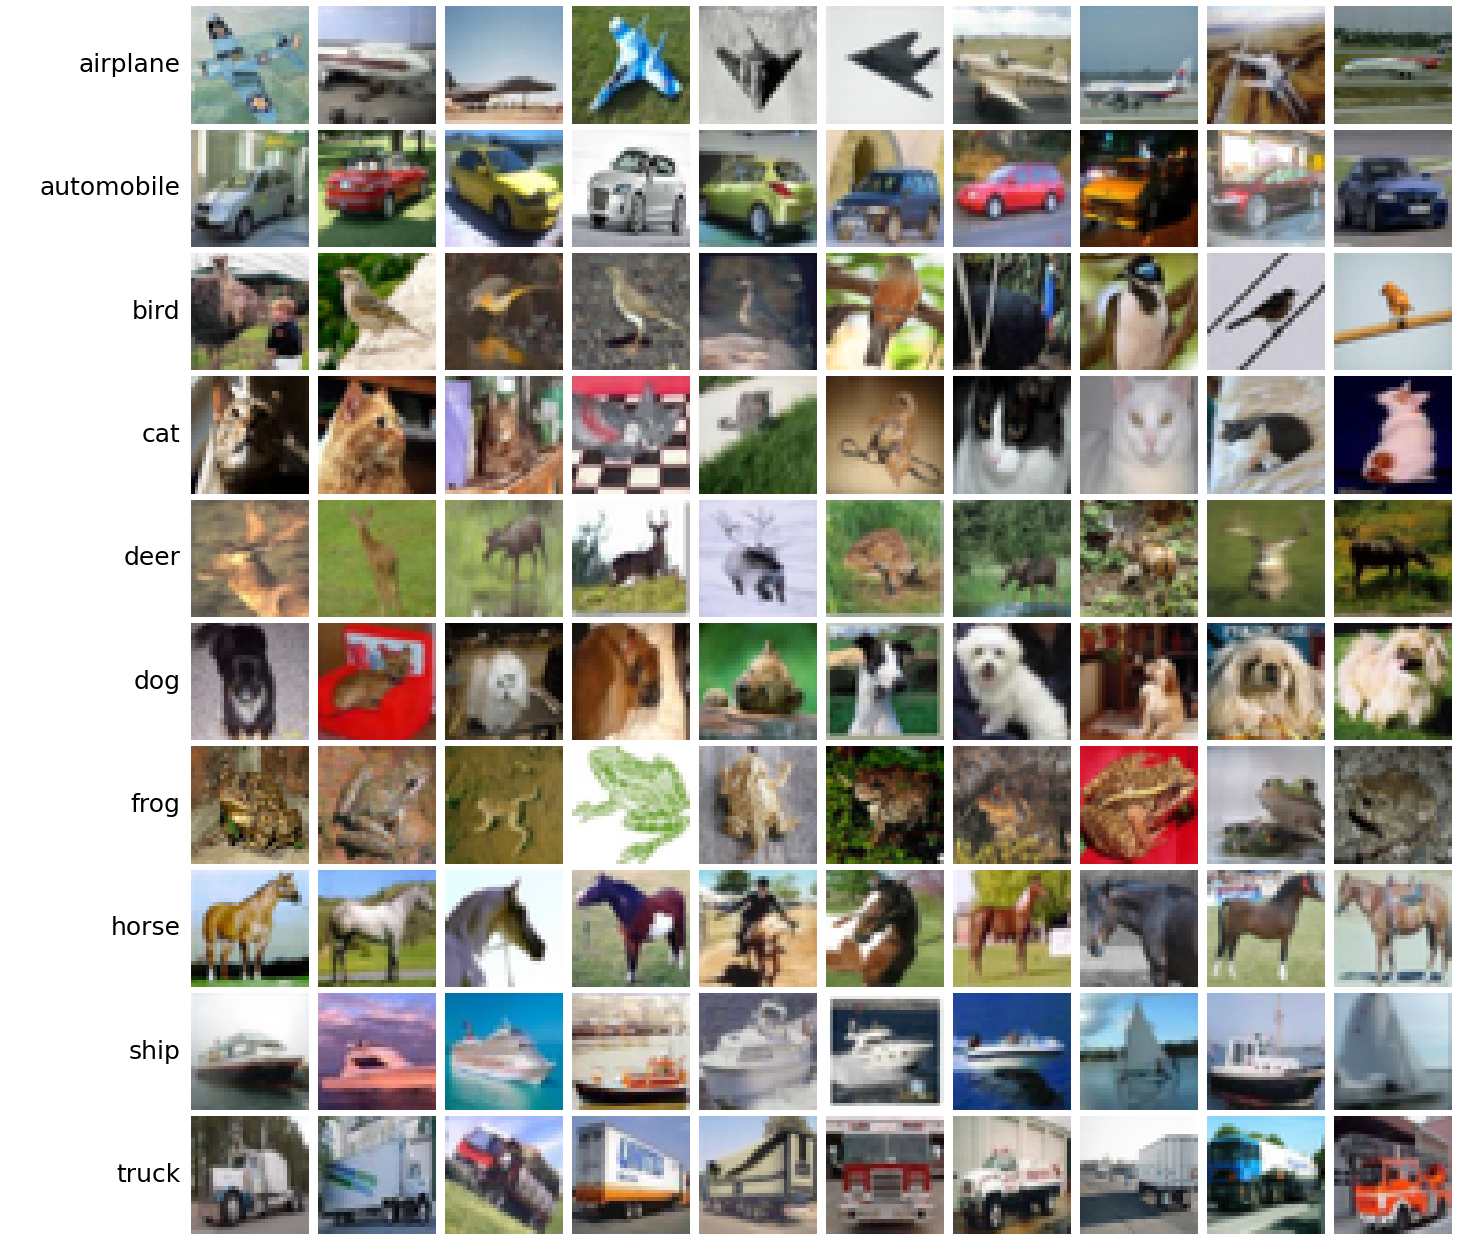
\includegraphics[width=0.8\textwidth]{cifar10_examples.png}
\caption{Ten random holdout images from each CIFAR-10 class.}
\label{fig:cifar}
\end{figure}

Each image is a $32 \times 32 \times 3$ array, i.e.\ a vector in $\mathbb{R}^{3072}$.
In this part we build a compressed representation of the images by performing PCA on the
raw pixels, and then test how well this representation supports classification by
training several neural networks on it.

\begin{question}[10]
Implement PCA: \texttt{fit\_pca}, \texttt{transform\_pca}, and
\texttt{reconstruct\_pca} (notebook Section 1A).
\end{question}

\begin{question}[10]
The notebook plots the variance explained by each principal component (on log--log
axes) and the cumulative explained variance against the number of components $k$, and
shows holdout images reconstructed from several values of $k$. In your report:
\begin{itemize}
  \item Describe how the variance explained by each component decreases with $k$, and
    what this means for the cumulative explained variance.
  \item Describe qualitatively what information the top principal components keep, and what they
    discard.
  \item Choose at least four values of $k$ to try in the rest of this part, and explain
    your choice.
\end{itemize}
Include any figures from the notebook that support your findings.
\end{question}

\begin{solution}
Your answer here.
\end{solution}

\begin{question}[5]
Implement at least two neural networks of increasing size as \texttt{nn.Module}
classes (notebook Section 1C).
\end{question}

\begin{question}[10]
Train each of your architectures on each of your values of $k$, and report:
\begin{itemize}
  \item A short description of each architecture, its number of parameters, and why you
    chose it.
  \item A table with the best epoch and the training and holdout accuracy for every
    combination, and the plot of accuracy against $k$. Mark the best combination.
\end{itemize}
Discuss the patterns you observe, including any overfitting. Explain them in terms of how
much information the representation contains as $k$ increases, and the capacity of each
network.
\end{question}

\begin{solution}
Your answer here.
\end{solution}

\subsection{Extra Credit: CNN (5 EC points)}

Train a convolutional neural network directly on the $32 \times 32 \times 3$ images (no
PCA) and report its holdout accuracy. You will need to write the model and training code
yourself. Compare it with your best model from this part, and explain why a CNN's
inductive bias may suit images better than an MLP on PCA features.

\begin{ecsolution}
Your answer here.
\end{ecsolution}

\section{Part 2: CLIP Features (20 points)}

In Part 1 the features came from the pixels of CIFAR-10 alone. Now we take features from
CLIP (Contrastive Language--Image Pre-training), a model pretrained on a very large
collection of images and text.

\subsection{Embeddings learned from pairs}

In Lecture 11 we learned embeddings whose geometry captures a property of the
data. In the clothing-style example, a Siamese CNN $\Phi$ maps each item image to a
vector, and training pulls together the embeddings of compatible pairs while pushing
apart the embeddings of incompatible pairs:
\[
  \argmin_\Theta \sum_{(i,j) \in D} L^+\big(\Phi(x_i), \Phi(x_j)\big)
  + \sum_{(i,j) \in \tilde D} L^-\big(\Phi(x_i), \Phi(x_j)\big).
\]
CLIP applies the same idea to pairs made of one image and one piece of text.

\subsection{The model}

CLIP has two encoders:
\begin{itemize}
\item an \textbf{image encoder} $f$, which maps an image $x$ to a vector $f(x) \in \mathbb{R}^{512}$,
\item a \textbf{text encoder} $g$, which maps a string $t$ to a vector $g(t) \in \mathbb{R}^{512}$.
\end{itemize}
Both outputs are normalized to unit length, so their inner product is a cosine
similarity:
\[
  s(x, t) = f(x)^\top g(t) \in [-1, 1].
\]
For now, don't worry about the architecture. Treat $f$ and $g$ as fixed functions.

\subsection{Training data and objective}

CLIP was trained on about 400 million (image, caption) pairs collected from the
internet. Training uses batches of $N$ pairs $(x_1, t_1), \dots, (x_N, t_N)$ ($N = 32{,}768$
in the paper). Within a batch, the caption $t_i$ is the positive for image $x_i$, and
the other $N-1$ captions in the batch are its negatives. Let
$S_{ij} = s(x_i, t_j) / \tau$, where $\tau$ is a learned temperature. The loss is
\[
  \mathcal{L} = -\frac{1}{2N} \sum_{i=1}^{N} \left[
    \log \frac{\exp(S_{ii})}{\sum_{j=1}^{N} \exp(S_{ij})}
    + \log \frac{\exp(S_{ii})}{\sum_{j=1}^{N} \exp(S_{ji})}
  \right].
\]
The first term is a softmax cross-entropy. For each image it poses an $N$-way
classification problem (which caption in this batch belongs to this image?), exactly
like multinomial logistic regression with the $N$ caption embeddings as the class
weight vectors. The second term is the same problem in the other direction (which
image belongs to this caption?). Minimizing $\mathcal{L}$ pulls each image towards
its own caption and pushes it away from the other captions in the batch, just as
$L^+$ and $L^-$ do above.

For more detail, see Sections~2.2 (the training data) and~2.3 with Figure~3 (the
objective and pseudocode) of Radford et al., ``Learning Transferable Visual Models
From Natural Language Supervision'', ICML 2021 (\url{https://arxiv.org/abs/2103.00020}).

\subsection{Questions}

In this part we use only the image encoder, treating $f(x)$ as a new feature vector for
image $x$, and we train the same classifiers as in Part 1 on it. The notebook extracts $f(x)$
for every CIFAR-10 image, after upsampling the $32 \times 32$ images to
$224 \times 224$.

\begin{question}[10]
The notebook trains every architecture from Part 1 on the CLIP embeddings
($d = 512$), reports a table of results, and plots the training and holdout loss over
the epochs. In your report:
\begin{itemize}
  \item Compare each architecture trained on CLIP features with the same architecture
    trained on PCA features in Part 1. Which features lead to faster convergence, and
    which to a higher ceiling?
  \item Compare the architectures on CLIP features only. Which converges fastest?
\end{itemize}
Include any figures from the notebook that support your answers.
\end{question}

\begin{solution}
Your answer here.
\end{solution}

\begin{question}[10]
Answer the following:
\begin{itemize}
  \item Compared with Part 1, how much does the choice of architecture change holdout
    accuracy on CLIP features, and on PCA features?
  \item Why do we observe this trend? Think about what job the classifier has to do,
    and how this follows from the way the two embeddings are obtained and from CLIP's
    pretraining.
\end{itemize}
\end{question}

\begin{solution}
Your answer here.
\end{solution}

\section{Part 3: Zero-Shot Classification (25 points)}

So far every classifier was trained on labeled CIFAR-10 images. CLIP's text encoder
allows classification without any labeled images. Write one text prompt per class,
e.g.\ $t_c = $ ``a photo of a dog.'', and predict the class whose prompt is most
similar to the image:
\[
  \hat y(x) = \argmax_{c} \; f(x)^\top g(t_c).
\]
This is a linear classifier, like logistic regression on CLIP features, except that the
weight vector for class $c$ is $g(t_c)$. The weights come from the text encoder instead
of being learned from labeled images. This is called zero-shot classification.
Sections~3.1.2 and 3.1.4 of the CLIP paper describe it and the effect of the prompt
wording.

\begin{question}[5]
Implement \texttt{zero\_shot\_classify} (notebook Section 3A).
\end{question}

\begin{question}[10]
A template is a prompt with a slot for the class name, such as
``a photo of a \{\}.''. The notebook evaluates a few templates on the holdout set.
\begin{itemize}
  \item Add at least \textbf{three} templates of your own. Report every template with
    its holdout accuracy. Which one is best, and which one is worst?
  \item Explain why, using what you know about the captions CLIP was trained on and
    about the CIFAR-10 images.
\end{itemize}
\end{question}

\begin{solution}
Your answer here.
\end{solution}

\begin{question}[10]
Zero-shot classification uses no labeled CIFAR-10 images. To measure how many labels it
is worth, the notebook trains logistic regression on only $n$ labeled CLIP embeddings per
class, for $n$ from 1 to 256.
\begin{itemize}
  \item Include the plot of holdout accuracy against $n$, with the accuracy of your best
    zero-shot template as a horizontal line. About how many labeled images per class is
    zero-shot classification worth?
  \item Does this number depend on the domain? Look at Figure~7 of the CLIP paper and
    discuss what you observe.
\end{itemize}
\end{question}

\begin{solution}
Your answer here.
\end{solution}

\pagebreak
\section{Part 4: Attribute Binding (20 points)}

Zero-shot classification works well when the classes differ in which objects are in
the image. Here we test whether CLIP also knows which attribute belongs to which object.
This is called attribute binding.

The notebook generates synthetic scenes. Every image contains two objects, each with a
color and a shape (5 colors and 4 shapes, and the two objects differ in both). For each image
we build three captions:

\begin{center}
\begin{tabular}{lll}
\hline
Caption & Example & What changed \\
\hline
True & a photo of a green triangle and a yellow square. & -- \\
Swapped & a photo of a yellow triangle and a green square. & colors swapped between objects \\
Control & a photo of a green triangle and a blue square. & one attribute not in the image \\
\hline
\end{tabular}
\end{center}

\noindent
The swapped caption uses exactly the same words as the true one. The control caption
mentions something that is not in the image.

\begin{question}[10]
Implement \texttt{two\_way\_zero\_shot} (notebook Section 4A). Report the accuracy of the true-vs-swapped and true-vs-control tests. Include the
histogram of margins $s(x, t_\text{true}) - s(x, t_\text{alt})$ and explain what it
shows.
\end{question}

\begin{solution}
Your answer here.
\end{solution}

\begin{question}[10]
Why does contrastive training produce this behavior? Read Sections~2.2--2.3 and
Figure~3 of the CLIP paper, and review the training details of the Siamese embedding in
Lecture 11 (in particular, why negative pairs are subsampled). In CLIP's loss, each
image must pick its own caption out of the other captions in its batch.
\begin{itemize}
\item What do those other captions typically look like for random web image--caption
  pairs?
\item How often would a batch contain a caption that differs from the correct one only
  in which attribute goes with which object?
\item What, then, does the model need to learn to make the loss small, and why does that
  explain your results?
\end{itemize}
\end{question}

\begin{solution}
Your answer here.
\end{solution}

\subsection{Extra Credit: Fixing Binding (5 EC points)}

Generate a training set of scenes and captions, and implement a fine-tuning pipeline
that improves CLIP's true-vs-swapped accuracy on held-out scenes, without losing
accuracy on the control test. You will need to write all of the code yourself. For
example, you could keep CLIP frozen and learn a matrix $A$ that defines a new similarity
$f(x)^\top A\, g(t)$, or fine-tune part of CLIP, using swapped captions as hard
negatives. Describe your method and report the swap and control accuracy before and
after.

\begin{ecsolution}
Your answer here.
\end{ecsolution}

\end{document}
